\documentclass[10pt]{article}
\newtheorem{define}{Definition}
%\newcommand{\Z}{{\mathbb{Z}}}
%\usepackage{psfig}
\usepackage{graphics}      % standard graphics specifications
\usepackage{graphicx} 

\oddsidemargin=0.15in
\evensidemargin=0.15in
\topmargin=-.5in
\textheight=9in
\textwidth=6.25in

\begin{document}
\input{preamble.tex}

%{lecture number}{lecture date}{Brendan Juba}{Your name}
\lecture{16}{October 27, 2016}{Brendan Juba}{Manil Bastola}
% The bare minimum guide to LaTeX
%
% (Lines beginning with the % are comments and don't appear in the output.)
%
% For the most part, you can simply enter plain text as you normally would.
% You are encouraged to break your notes up into sections using
%
% \section{Name of Section}
%
% and subsections
%
% \subsection{Name of subsection}
%
% and perhaps even subsubsections (you get the idea). Sections etc. are numbered
% for you automatically. There is also a \paragraph{Title of paragraph} command 
% that allows you to title a paragraph (without numbering).
%
% You can use math mode inline by suspending the math commands in $'s
% as in, $1+1=2$. Please use this whenever you discuss values or variables in
% your text. There are also more advanced equation environments and math modes.
% You will want to find a more detailed reference to help you use these.
%
% The file preamble.tex defines a number of environments for theorems,
% definitions, and proofs, as well as commands for use in math mode.
% When using the definition environment, be sure that you emphasize the term
% being defined, {\em like so}.
%
% You can automatically refer to any numbered objects -- sections, theorems,
% definitions, etc. -- by first using the \label{name_of_object} command
% (immediately following the command that creates the item) to assign it a
% name. Subsequently, \ref{name_of_object} will be substuted by the number
% LaTeX assigns when it compiles your document. You have to run LaTeX twice
% to get these placed correctly.

%%%% body goes in here %%%%
\ \\
$\bf{Today's\ topics:}$
\begin{itemize}
  \item``Common Sense" knowledge and reasoning
 \item  Non-monotonic reasoning and reasoning with examples
\end{itemize}
\ \\
$\bf{Two\ types\ of\  knowledge}$
\begin{enumerate}
\item Acquired knowledge : Deduced/Declarative and Inductively learned (from personal experience or a knowledge that everyone knows), and
\item Innate knowledge
\end{enumerate}
$\bf{Common\ Sense}$\\
``Common sense" is a variety of tacitly shared knowledge that we rely on in an action or communication.\\
Common sense $\approx$ Innate  knowledge + Inductively learned  knowledge that everyone knows.\\
\begin{figure}[!ht]
\centering
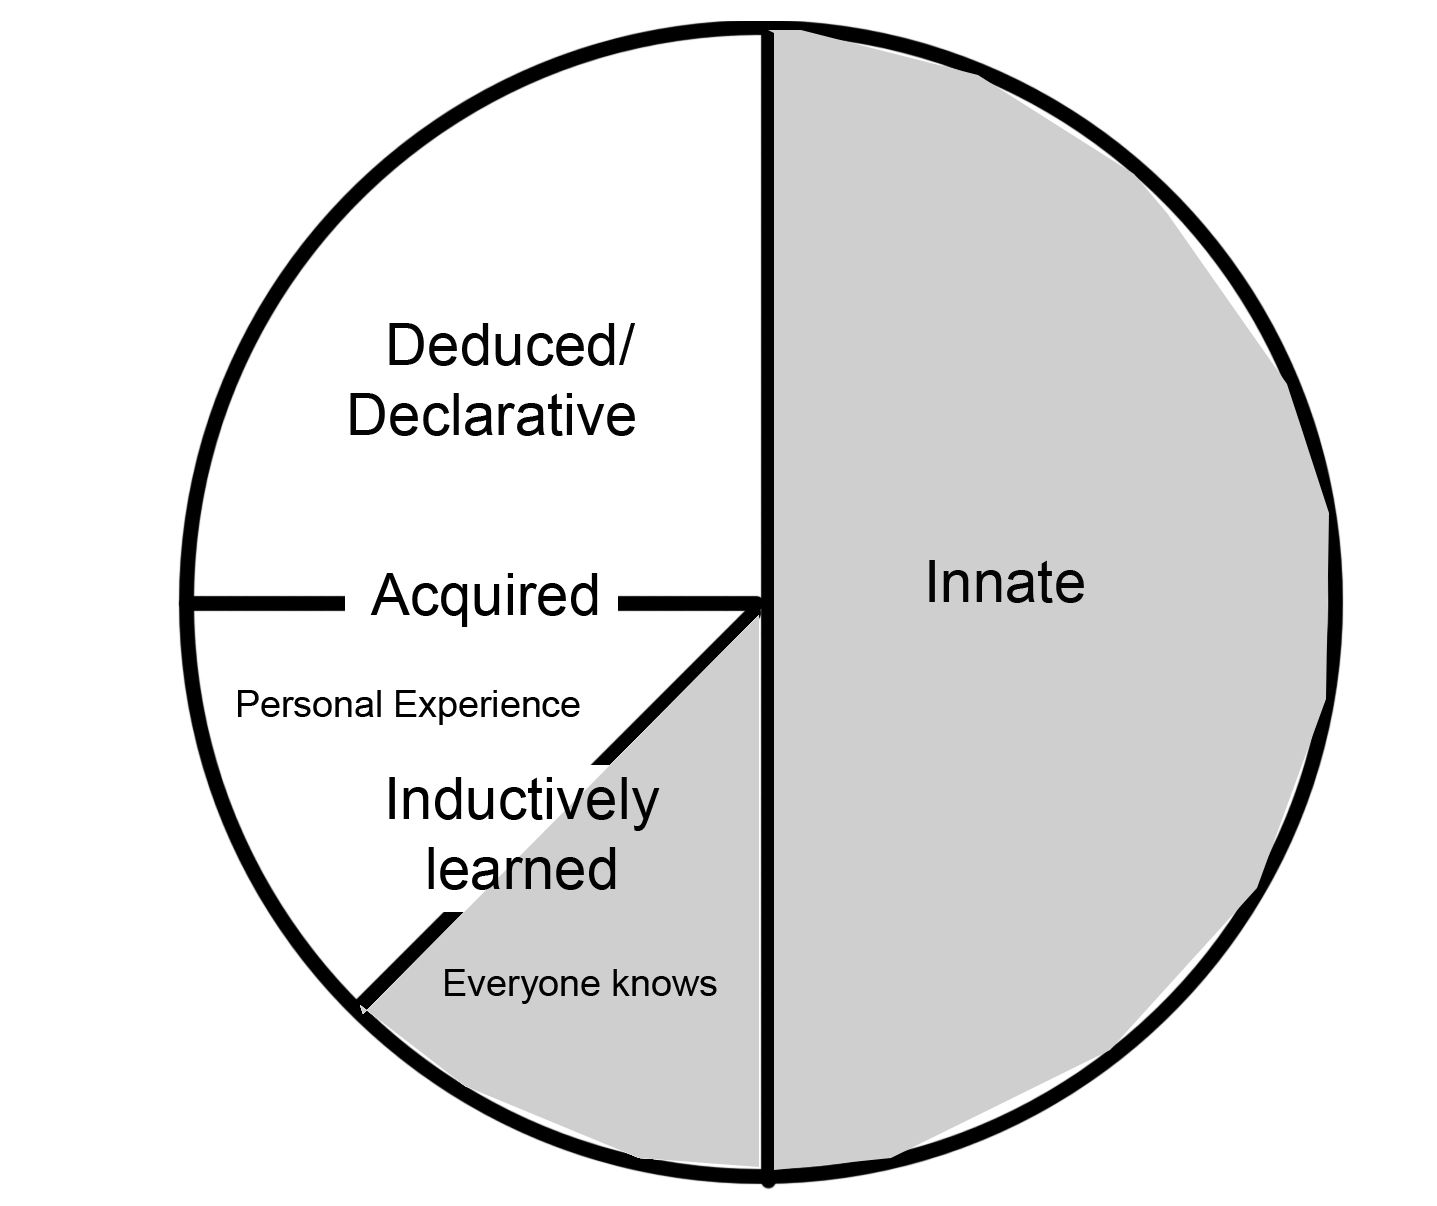
\includegraphics[width=7cm]{common}
\caption{\it Types of knowledge with common sense represented in the shaded region.} 
\end{figure}
\\
\\
Some questions that we do not know answers to:
\begin{itemize}
  \item How much of what we know is innate? 
 \item What knowledge is innate?
\end{itemize}
Cognitive psychology has identified several domains that seem to be innate:
\begin{itemize}
  \item Space \& Objects e.g. ideas about ``persistence",``identity", etc.
 \item Naive physics
\item Naive psychology (intentions and emotions, etc)
\item Quantitative reasoning (more vs less, small numbers arithmetic, etc.)
\end{itemize}
Innate domains are not generally present at birth but are developed according to a fixed schedule. It seems unlikely that some of these could be learned. For example, the relatively complex models of naive psychology. In other cases, for example naive physics, it seems that perhaps simulation or other ``non-logical" method are useful to answer such questions.
\\
\\
$\bf{Non-monotonic\ Reasoning}$\\
In common sense reasoning, it is important to be able to ``leap to conclusions". For example, if I place a book in my bag, then in the absence of the evidence to the contrary, I ``know" (presume) my book is still there. If I open the bag and the book is not there - maybe it fell out, maybe someone took it out, etc. then I am forced to ``retract" that the book is in the bag.\\
\\
Contrast this with classical logic: As I learn more i.e. add representations to my knowledge base KB, only more representations become valid for the KB, desirable from the KB and so on. In this sense, classical logic is monotonic, but common sense reasoning is not.\\
\\
Some key questions:
\begin{itemize}
  \item Which conclusions that aren't entailed should we reach?\\
( The common sense's ``Law of inertia" i.e. ``everything is presumed to remain in the state in which it is" is a good candidate. What else?)
\item How do I reach them efficiently?\\
\end{itemize}
Many of the properties we wish to  assert are similar to the kinds of rules we considered in agnostic learning.
For example, birds fly, games are won or lost, etc.
Reasoning with examples using ``filtering" mechanism captures at least some of the behavior for learned knowledge.\\
\\
Lets suppose we had some examples drawn from a distribution $D$, and we ``filtered" out the examples where $bird(x)\ne 1$. This has the affect of simulating draws from the conditional distribution $D/bird$ if $bird(x)=1, and 0$ otherwise. Here, $D/bird(x) = D(x)/Pr(bird)$.
\\
\begin{table}[ht!]
\centering
    \begin{tabular}{|r|r|r|r|r|r|}
    \hline
bird & fly & has-beak & red & purple & penguin\\
   \hline
1&1&1&0&0&0\\
  \hline
1&1&1&1&0&0\\
  \hline
1&0&1&0&0&1\\
  \hline
1&1&1&0&0&0\\
  \hline
1&0&1&0&0&1\\
  \hline
1&1&1&1&0&0\\
  \hline
1&1&1&0&0&0\\
  \hline
  \end{tabular}%
  \caption{Sample truth table for $bird(x)$ with example attributes such as fly, has-beak etc.}
\end{table}% 
\\
Suppose we are willing to tolerate $\epsilon = 1/3$ error. Do we conclude that ``fly" is $1-\epsilon$ valid?\\
$=\frac{1}{7}\sum_{i=i}^{7}fly(x^{(i)}) = \frac{5}{7}\ge\frac{2}{3}$, hence valid.\\
\\
How about $bird \land red$?\\
$=\frac{1}{7}\sum_{i=i}^{7}fly(x^{(i)}) = 1 \ge\frac{2}{3}$, so red birds fly.\\
\\
How about $bird \land penguins$?\\
$=\frac{1}{7}\sum_{i=i}^{7}fly(x^{(i)}) = 0 <\frac{2}{3}$, so cannot conclude ``fly". But actually, 
$\frac{1}{7}\sum_{i=i}^{7}\neg fly(x^{(i)}) = 1 \ge\frac{2}{3}$, so birds that are penguins conclude ``do not fly".\\
\\
If we consider $bird \land penguin \land has\ beak$, still $\neg fly$ holds.\\
\\
What about purple penguins?\\
Here, we have no example. Hence, we are unclear how to decide. If $Pr[\ penguin\land purple\ ]= 0$, then the conditional distribution $D/purple\ penguin$ is not well-defined. Hence, we shouldn't come to any conclusions.\\
\\
$\bf{Common\ issues\ in\ common\ sense\ representations}$
\\
\begin{enumerate}
\item $\bf{Qualification\ problem:}$\\
It is impossible to list out all of the conditions that are necessary for some ``natural concept" to be true.\\
\\
For example, take ``birds fly". To account for penguins, we might assert that ``birds that are not penguins fly". How about dead birds?. To accommodate this we may say ``Birds that are not dead and are not penguins fly". However, how about birds in other planets with high gravity? and so on...\\
\\
We avoided this problem in PAC semantics by allowing the rule to fail $w.p.\ \epsilon$ for some unexpected reason.\\
\item $\bf{Ramification\ Problem:}$\\
Especially when we reason about action and change, one small change or a piece of information can have many consequences. For example, if we are loading a crate on to a boat and the boat sails away. Then the crate goes with the boat along with everything inside the crate. \\
\\
We need to efficiently derive the many conclusions about things changing while respecting the law of inertia. On reasoning with examples, at least the attributes that are represented are ``automatically" updated when we filter.\\
\item $\bf{Elaboration\ tolerance:}$\\
When we discover a new exception to a rule, we'd like to be able to incorporate the knowledge of this exception without needing to modify every rule in the KB i.e. the updates should be ``efficient". In reasoning with examples we simply add exceptional example to a list and reason as usual with the larger list. \\
\end{enumerate}
$\bf{Classical\ approach\ to\ common\ sense}$\\
\\
Produce a KB containing all common sense knowledge. Estimates of the size of this KB run on the order of $0.5- 3.4\ Gb$ $\approx 10^7-10^8$  ``elements" of knowledge. Curating such a KB manually is daunting. Most prominent effort still only contains 7M assertions with about 3M terms in 3 years.\\
\begin{itemize}
  \item Automated Collection (For example. from the web)\\
	KNEXT mined $10^8$ ``factoids" from Wikipedia  and blogs. But we are after really mundane knowledge such as ``water needs a container",etc. which is rare to find in web.
\item Crowd sourcing\\
 Open Mind Common Sense (OMCS) project grew from $4.5 \times 10^5$ facts to $>1M$ in 2014. Still may take $>100$ years with this rate.
\end{itemize}
How do we acquire so much knowledge so quickly?\\
How can we use such a KB so efficiently?\\
\\
Reasoning with examples by contrast may ``implicitly" encode the answers to (exponentially) many queries in relatively few examples.\\
Main problem is that the method relies heavily on complete information.\\
\\
Next time, we will extend reasoning with examples to work with complete information. 
\end{document}

